\documentclass{article}
\usepackage[utf8]{inputenc}
%\usepackage{mathabx}
%\usepackage{amsopn}
\usepackage{cite}
\usepackage{graphicx}
\usepackage{float}
\usepackage{caption}
\usepackage{amsmath}
\setlength\parindent{0pt}
\graphicspath{{C:\Users\Pruthvi\git\phmehta95\thesis\thesis}}




\title{Systematic uncertainty calculations}

\begin{document}
\maketitle



\section{Systematic uncertainty calculation methodology}\label{systmethod}


The systematic uncertainities for this analysis are calculated using the probablity distribution functions of each quantity appearing in the formula for the mean neutron multiplicity, which is given by:

\begin{equation}
    M=\frac{\# n_{\text {det }}-R \times \# \nu_{\text {det }}}{T} \frac{1}{\# \nu_{\text {det }}}
 \label{multiplicity}
\end{equation}



By random sampling the probability distribution functions for each of the terms in Equation \eqref{multiplicity} one can calculate the multiplicity probability distribution functions for both the statistical uncertainty and the systematic uncertainty. The statistical uncertainty for the value for the multiplicity is related to the variation in the number of detected neutrons, while the systematic uncertainty is related to the variation on the tagging efficiency and the background rate. The total search time for the tagged neutrons is dependent on the number of "windows" in which the neutron is searched for in, and therefore the term for the number of detected neutrinos. Because any variation on the number of neutrinos which are detected is unrelated to the value for the mean neutron multiplicity, calculating a probability mass function for the number of neutrinos is uneccessary. 

A Poissonian distribution is used to model the distribution for the number of detected neutrons, due to its value being approximated by counting the positives in the timing window that the neutron tagging search is carried out in. The mean value of this Poisson distribution is denoted in Equation \eqref{poissonuncertainty}.
\newline
\begin{equation}
    P M F\left(\# n_{\text {det }}\right)=\frac{1}{\left(\# n_{\text {det }}\right) !}\left\langle \# n_{\text {det }}\right\rangle^{\# n_{\text {det }}} e^{-\left\langle \# n_{\text {det }}\right\rangle}
\label{poissonuncertainty}
\end{equation}
\newline
Regarding the background rate, this is estimated from dummy spill data, but it's error is associated with the statistical variation of the Monte Carlo size that the backround rate is associated with, and secondly the change of the background rate value during the SK-V period. The statistical variation of the MC is modelled using a Gaussian, while the uncertainty relating to time variation is characterised by its own probability distribution function. In contrast, the tagging efficiency is model dependent and has systematic uncertainties relating to this. The two ways in which the systematic error are estimated are either using MC re-weighting or MC regeneration.
\newline
For the MC-reweighting approach, weights are applied to a quantity and the tagging efficiency of the re-weighted MC is extracted. The general methodology is to have the input of a model (given by a set of parameters) and to vary them one by one and then calculate the reweighted tagging efficiencies - the set of relative discrepancies $\delta_{i}$ are computed from this set of reweighted tagging efficiencies $T_{i}$ and the nominal tagging efficiency $T_{nom}$ using Equation \eqref{tageffdiscrep}.
\newline
\begin{equation}
    \delta_{i}=\frac{T_{i}-T_{\text {nom }}}{T_{\text {nom }}} \quad i \in\{\text { parameters }\}
\label{tageffdiscrep}
\end{equation}
\newline

These relative discrepancies $\delta_{i}$ are used to calculate the one indivdual discrepancy $\delta_{reweighted}$ that would describe the final deviation from the nominal tagging efficiency $T_{nom}$ due to the systematic error. $\delta_{reweighted}$ describes the model which has been produced through 1$\sigma$ variations of these parameters, therefore the final probability distribution function which describes the deviation from the nominal MC has a Gaussian distribution with the standard deviation being equal to $\delta_{reweighted}$. 
\newline
The other method to estimate the systematic error on the tagging efficiency is the method of Monte Carlo regeneration. This is carried out by varying a parameter then regenerating the whole Monte Carlo and then extracting the tagging efficiency - therefore unlike with MC re-weighting there is no set of discrepancies $\delta_{i}$ but instead two single discrepancies $\delta_{min}$ and $\delta_{max}$. The resulting probability distribution which describes the deviation from the nominal Monte Carlo is a Gaussian which has the mean and standard deviation relating to the discrepancies shown in Equation \eqref{mcregengauss}.
\newline

\begin{equation}
\left\{\begin{array}{l}
\mu=\frac{\delta_{\max }+\delta_{\min }}{2} \\
\sigma=\frac{\delta_{\max }-\delta_{\min }}{2}
\end{array}\right.
\label{mcregengauss}
\end{equation}


\section{Neutrino beam flux uncertainty}

The uncertainty on neutrino beam fluxes can also be evaluated by looking at the dependence of the tagging efficiency on the flux variations. The beam fluxes for the four flavour modes 
$\left(\nu_{e} \overline{\nu_{e}} \nu_{\mu} \overline{\nu_{\mu}}\right)$ have the fractional uncertainties given for each mode, FHC and RHC. The binned uncertainties are shown in Figure .


Each individual bin for the flux is increased/decreased by its error, the Monte Carlo re-weighting method is then used to extract the taggging efficiency for each flux bin, and Equation \eqref{nubeamfluxerror} is used to calculate the fractional uncertainty.
\newline
\begin{equation}
    \delta_{i}(\pm \sigma)=\frac{T_{i}(\pm \sigma)-T_{\text {nom }}}{T_{\text {nom }}} \quad i \in\{\text { each flux bin }\}
\label{nubeamfluxerror}
\end{equation}
\newline
Figure \ref{fig:fluxuncertainty} shows the fractional errors calculated from the reweighted Monte Carlo, with the red bars showing the -1$\sigma$ variation and the blue bars showing the +1$\sigma$ variation. Table \ref{table:systuncertaintytable} contains the value for the total fractional uncertainty resulting from the neutrino beam flux, which was calculated using Equation \eqref{summingfluxuncertainty}, where the maximum value between the increased and decreased discrepancy is taken and summed over to produce the final neutrino flux beam uncertainty value.
\newline

\begin{equation}
    \delta_{\nu \text { flux }}=\sum_{i \in\{\text { bins }\}} \max \left[\left|\delta_{i}(+\sigma)\right|,\left|\delta_{i}(-\sigma)\right|\right]
 \label{summingfluxuncertainty}   
\end{equation}

\begin{figure}[h!]
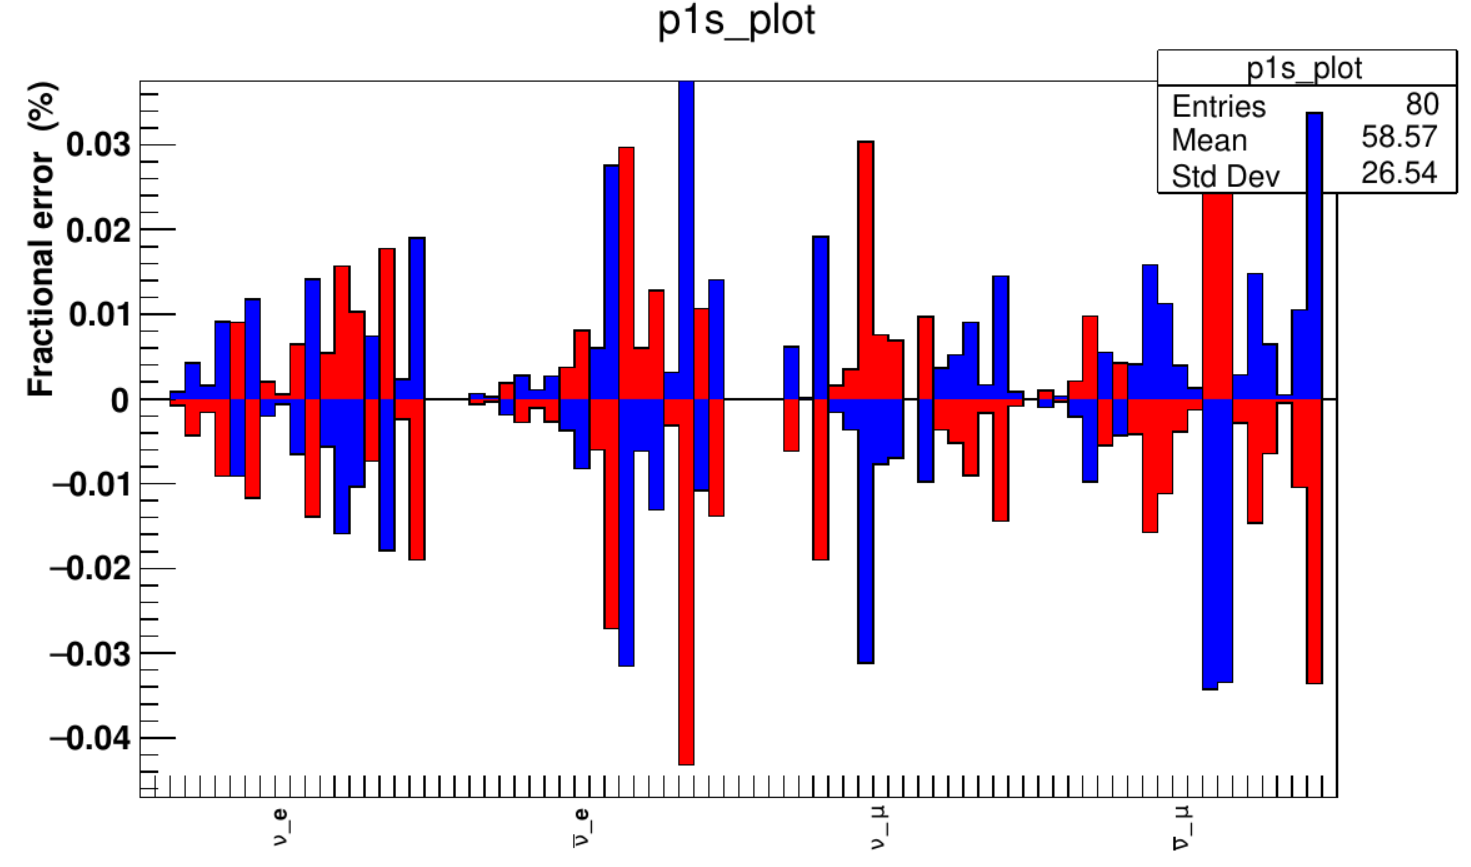
\includegraphics[scale=0.4]{flux_uncertainty.png}
\caption{Tagging efficiency fractional uncertainties caused by neutrino beam flux discrepancies. From left to right the sections in this plot are comprised of the beam fluxes elements of $\left(\nu_{e} \overline{\nu_{e}} \nu_{\mu} \overline{\nu_{\mu}}\right)$ respectively.}
\label{fig:fluxuncertainty}
\end{figure}

\section{Neutrino cross section uncertainty}

A group of default neutrino cross section values are used to make up the nominal Monte Carlo from which the tagging efficiency is calculated. The values of the parameters that determine the cross sections are shown in Table \ref{xsectable}. Each of the parameter values relate to a specific interaction type and are either a normalisation parameter or a paramater which show a kinematic dependence. The re-weighting method mentioned in Section \ref{systmethod} is used to reweight the nominal Monte Carlo on an event by event basis with each parameter value being increased and decreased by its uncertainty, and for each reweighted Monte Carlo the equivalent tagging efficiency value is extracted. Equation \eqref{xsectageff} shows how the fractional discrepancies are extracted from the nominal and reweighted tagging efficiency values.

\begin{equation}
\delta_{i}(\pm \sigma)=\frac{T_{i}(\pm \sigma)-T_{\text {nom }}}{T_{\text {nom }}} \quad i \in\{\text { parameters }\}
\label{xsectageff}
\end{equation}

Figure \ref{fig:xsecuncertainty} shows the reweighted Monte Carlo fractional uncertainty plotted for the FHC sample. Since this sample contains a lot of NCother interactions, the uncertainty for this interaction type is greater than for the others.

$$
\begin{array}{llll}
\hline & & & \\
\text { Parameter } & \text { Interaction } & \text { Type } & \text { Value } \\
& & & \\
p_{F}^{O} & \mathrm{CCQE} & { }^{16} \mathrm{O} \text { Fermi momentum } & 225 \pm 31 \mathrm{MeV} / \mathrm{c} \\
E_{B}^{O} & \mathrm{CCQE} & { }^{16} \mathrm{O} \text { binding energy } & 27 \pm 9 \mathrm{MeV} \\
M_{A}^{C C Q E} & \mathrm{CCQE} & \text { Axial mass } & 1.2 \pm 0.41 \mathrm{GeV} / \mathrm{c}^{2} \\
2 p 2 h & & & \\
C_{A S}^{R E S} & 2 \mathrm{p} 2 \mathrm{~h} & \text { Normalization par. } & 1.0 \pm 1.0 \\
M_{A}^{R E S} & \mathrm{CC} \text { and } \mathrm{NC} 1 \pi & \text { Axial form factor } & 1.01 \pm 0.12 \\
B G_{A}^{R E S} & \mathrm{CC} \text { and NC1 } \pi & \text { Axial mass } & 0.95 \pm 0.15 \mathrm{GeV} / \mathrm{c}^{2} \\
\mathrm{CC} \text { other } & \mathrm{CC} \text { and } \mathrm{NC} 1 \pi & \mathrm{I}=1 / 2 \text { continuum background } & 1.3 \pm 0.2 \\
\mathrm{CC} \text { coherent } & \mathrm{CC} \text { other } & \text { E-dependent par. } & 0.0 \pm 0.4 \\
\mathrm{NC} \text { other } & \mathrm{CC} \text { coherent } & \text { Normalization par. } & 1.0 \pm 0.3 \\
\mathrm{NC} \text { coherent } & \mathrm{NC} \text { other } & \text { NC-dependent par. } & 1.0 \pm 0.3 \\
& & \text { Normalization par. } & 1.0 \pm 0.3 \\
\mathrm{FS} e^{-} \text {Bremsstrahlung } & \mathrm{CC} \nu_{e} & \text { Normalization par. } & 1.00 \pm 0.03 \\
\hline
\end{array}
\label{xsectable}
$$

\begin{figure}[h!]
    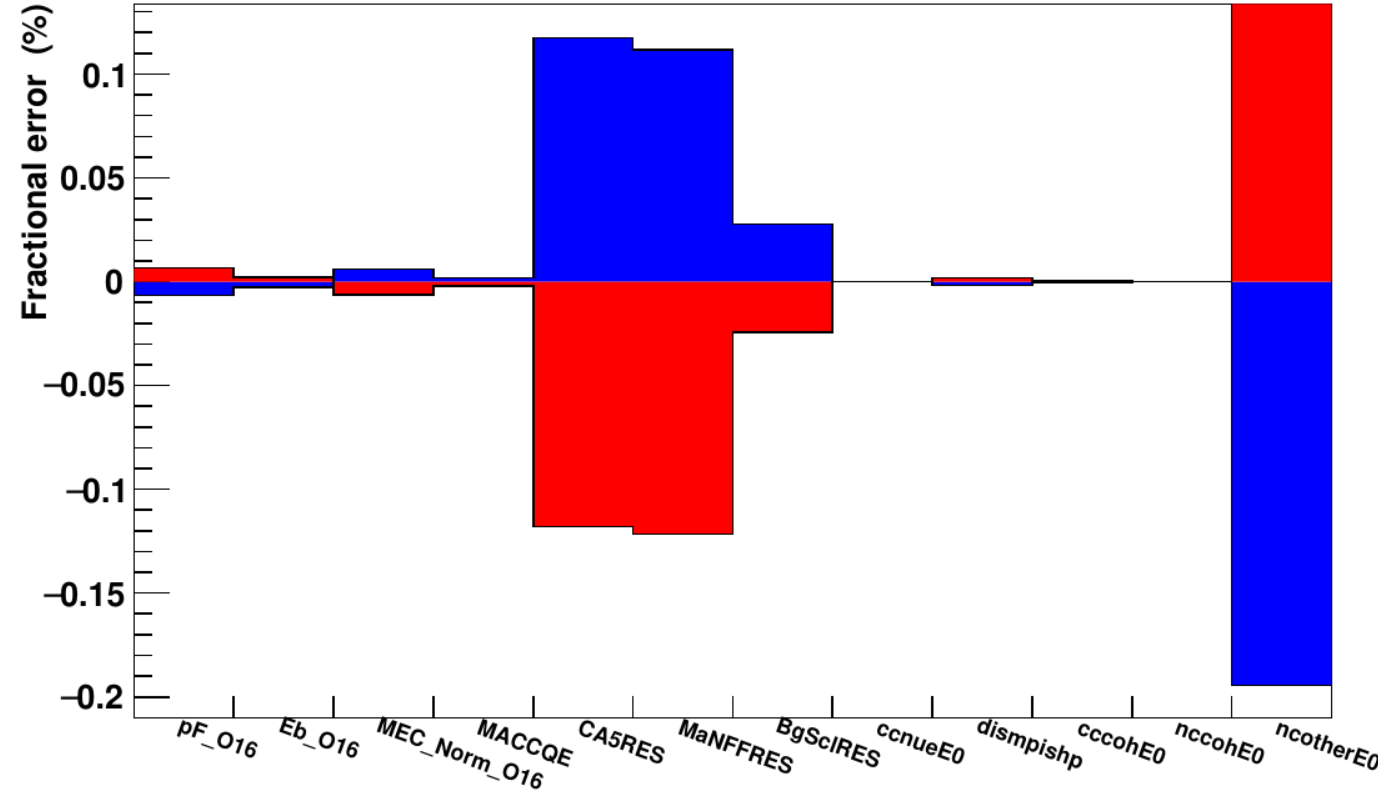
\includegraphics[scale=0.4]{xsec_uncertainty.png}
\caption{Tagging efficiency fractional uncertainty caused by the cross-section parameters variations for the FHC mode}
\label{fig:xsecuncertainty}
\end{figure}

\Section{Pion final state interaction (FSI) and secondary interaction (SI) uncertainties}




\end{document}